\section{Ubiquitous Language}

La seguente tabella mostra l'\textit{Ubiquitous Language} del dominio in analisi.

\begin{table}[H]
    \centering
    \begin{tabular}{|l|p{.8\textwidth}|}
        \hline
        \textbf{Termine} & \textbf{Definizione}\\
        \hline
        \ul{MicroCity}{Zona con estensioni spaziale e temporale limitate frequentata da ospiti interessati alle attività al suo interno.}
        \ul{Guest}{Persona interessata alle attività messe a disposizione nella \textit{MicroCity}.}
        \ul{Group of Guests}{Insieme di ospiti interessati alle stesse attività messe a disposizione nella \textit{MicroCity}.}
        \ul{Activity}{Servizio o evento che si svolge all'interno della \textit{MicroCity} che può soddisfare un certo numero di persone con una certa frequenza in base alla sua \textit{Duration}. Un'attività ha un \textit{Time Period} predefinito che ne stabilisce inizio e fine di operatività. Inoltre, può essere: statica, ovvero che non può essere riposizionata; o dinamica, che può spostarsi dove necessario o utile.}
        \ul{Service}{Tipologia di attività offerta agli ospiti all'interno della \textit{MicroCity}. Un servizio rimane continuamente operativo, permettendo ai \textit{guest} di fruirne in qualsiasi momento.}
        \ul{Event}{Tipologia di attività offerta agli ospiti della \textit{MicroCity}. Un evento ha luogo in un momento specifico e viene effettuato una sola volta, dopo la quale non è più disponibile.}
        \ul{Benefit From}{L'atto di soddisfare le necessità degli ospiti da parte delle attività.}
        \ul{Time Period}{Arco temporale di operatività di una \textit{Activity}, definito da un inizio e una fine.}
        \ul{Duration}{Tempo impiegato da un'attività per soddisfare le necessità di uno o più ospiti.}
        \ul{Wearable}{Dispositivo posseduto da ogni ospite o gruppo di ospiti che permette di interagire con la \textit{MicroCity}.}
        \ul{Boundary}{Perimetro fisico che definisce i confini della \textit{MicroCity}.}
        \ul{Worker}{Operatore interno alla \textit{MicroCity}. Non fruisce delle attività, ma può gestirle.}
        \ul{Suggestion}{Proposta di partecipazione ad una attività in cambio di un reward.}
        \ul{Suggest}{Azione di inviare Suggestion agli ospiti per incentivarli a partecipare alle attività.}
        \ul{Reward}{Vantaggio ricevuto dagli ospiti a seguito del compimento di una certa azione. Può essere concesso dalle attività per incentivare gli ospiti a seguire comportamenti specifici.}
        \ul{Map}{Rappresentazione della \textit{MicroCity} contenente informazioni utili agli ospiti riguardo alle posizioni delle attività. Può fornire indicazioni sui percorsi che collegano le attività.}
        \ul{Route}{Percorso che collega delle attività.}
        \ul{Waiting Time}{Tempo che gli ospiti attendono prima di poter fruire di un'attività.}
        \ul{Queue}{Coda di ospiti che si forma a causa dei lunghi tempi di attesa.}
        \ul{Fee}{Somma in denaro che gli ospiti devono pagare per accedere alla \textit{MicroCity} e/o per fruire delle attività.}
    \end{tabular}
    \caption{Ubiquitous language dell'ambito \textit{MicroCity}.}
    \label{tab:ul}
\end{table}

\section{Modello del dominio}\label{sec:modello-del-dominio}

A seguito della definizione dei concetti del dominio, di seguito sono illustrati alcuni diagrammi che mostrano le relazioni
tra essi.

In figura~\ref{fig:domain-overview} vengono mostrati i principali elementi che costituiscono la \textit{Micro City}.
In particolare, la \textit{Micro City} si compone di più \textit{Guest} che possono usufruire delle \textit{Activity} in essa
contenute.
Ogni \textit{Guest} possiede un \textit{Wearable} grazie al quale interagisce con \textit{Micro City}; un insieme di
più \textit{Guest} definisce il \textit{GroupOfGuest}.
Una \textit{Activity} può generare più \textit{Reward} che vengono ricevuti dai \textit{Guest} o \textit{GroupOfGuest}.

\begin{figure}[H]
    \centering
    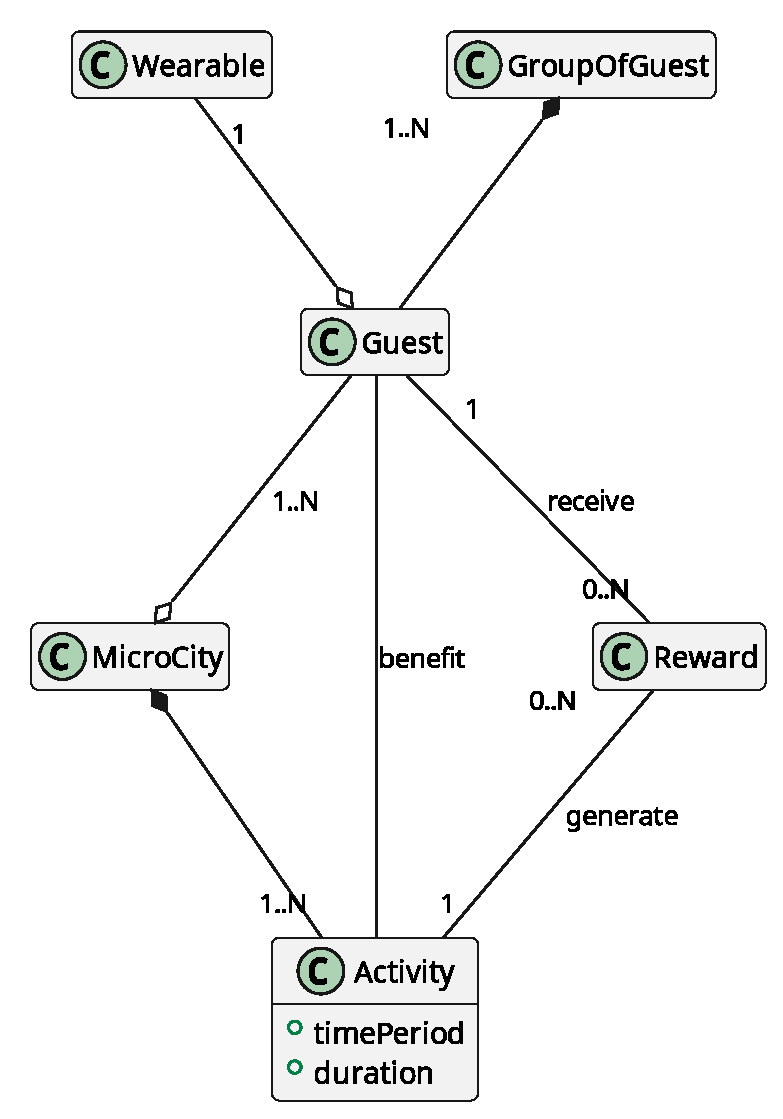
\includegraphics[width=0.55\textwidth]{./img/domain_overview-0}
    \caption{Diagramma delle classi che modella il dominio della \textit{Micro City}.}
    \label{fig:domain-overview}
\end{figure}

\newpage

In figura~\ref{fig:micro-city} viene mostrato un diagramma che rappresenta l'organizzazione della \textit{Micro City}.
Quest'ultima infatti, è composta da una \textit{Map}, un \textit{Oracle} e più \textit{Worker}.
Inoltre, sia le \textit{Activity} che la \textit{Micro City} potrebbero richiedere una \textit{Fee}, ovvero un compenso per
poter accedervi.
Sono modellati due tipologie di \textit{Activity}: \textit{Service} rappresenta un servizio generico continuamente operativo;
\textit{Event} rappresenta un evento attivato in un memento specifico con una durata.
\textit{Queue} rappresenta il tempo di attesa per poter accedere a una \textit{Activity}.

\begin{figure}[H]
    \centering
    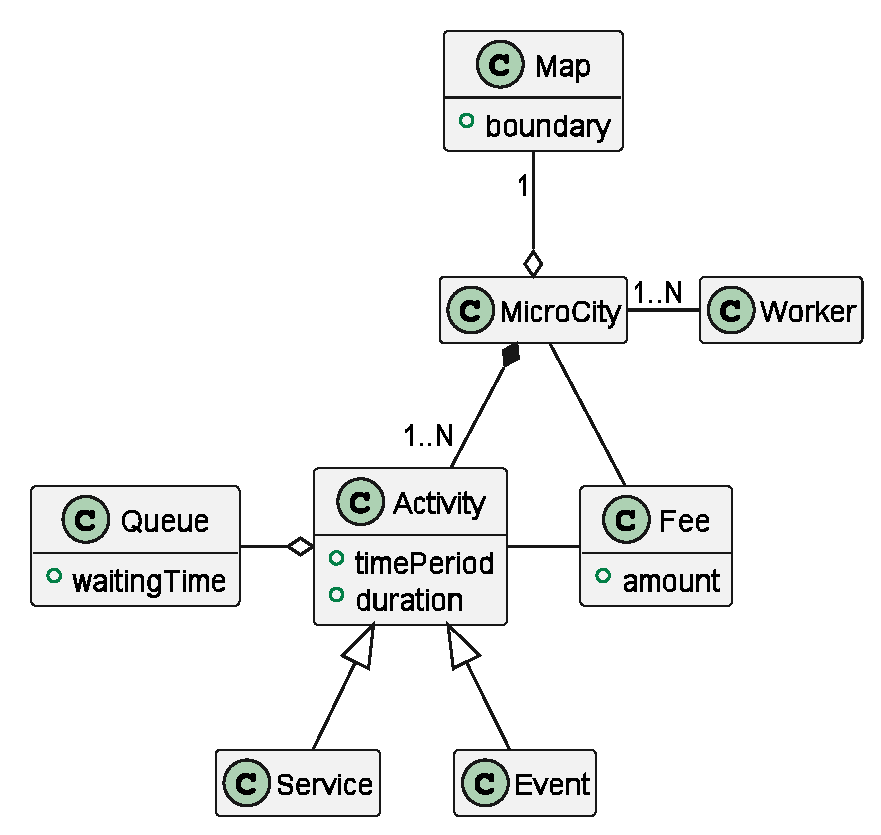
\includegraphics[width=0.7\textwidth]{./img/micro_city-0}
    \caption{Diagramma delle classi che modella l'organizzazione della \textit{Micro City}.}
    \label{fig:micro-city}
\end{figure}

\newpage

In figura~\ref{fig:reward} è mostrato il diagramma di sequenza che rappresenta l'ottenimento di un reward da parte di un ospite.

\begin{figure}[H]
    \centering
    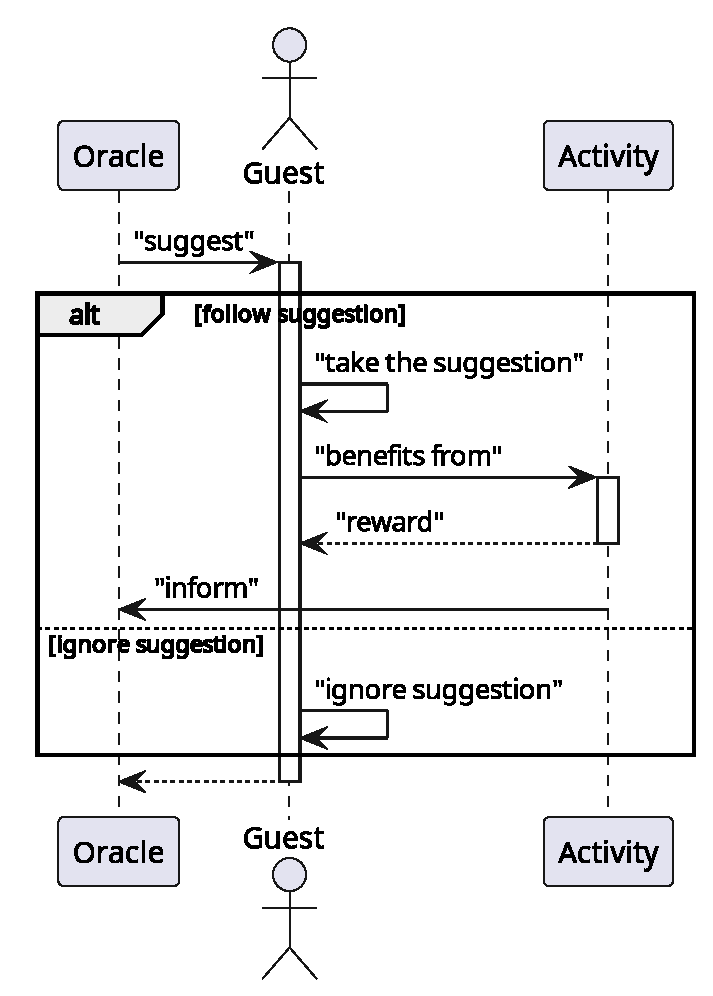
\includegraphics[width=0.6\textwidth]{./img/reward-0}
    \caption{Diagramma di sequenza che mostra il comportamento generico dei reward.}
    \label{fig:reward}
\end{figure}

\newpage
